\scanpage{14}
c)
\[
\begin{aligned}
\unsure{\mathfrak{S}|\mathcal{S}}_4&\simeq\operatorname{Aff}(2,\mathbb{F}_2)\simeq\operatorname{GP}(1,\mathbb{F}_3)\\
\unsure{\mathfrak{A}|\mathcal{A}}_4&\simeq\operatorname{Aff}(1,\mathbb{F}_4)\qquad ?
\end{aligned}
\]

d)
\[
\begin{aligned}
\mathfrak{S}_5&\simeq\operatorname{GP}(1,\mathbb{F}_5)\\
\mathfrak{A}_5&\simeq\operatorname{GP}(1,\mathbb{F}_4)
\end{aligned}
\]

Quelques groupes classiques sur un corps $k$

\diagram{\(\left.
\begin{tikzcd}[ampersand replacement=\&,column sep=small,row sep=1em]
1\arrow[r] \& k^*\arrow[r] \& \operatorname{Gl}(V)\arrow[r] \&\operatorname{GP}(V)\arrow[r,dash]\&1\\
1\arrow[r] \& k^*\arrow[r,dash] \&\operatorname{Gl}(n,k)\arrow[r] \&\operatorname{GP}(n-1,k)\arrow[r]\&1
\end{tikzcd}
\right\}\;\text{ne \unsure{splitte} pas en général}\)}

% slanted left-margin note; the enclosure has small open joins.
\reversemarginpar
\margin{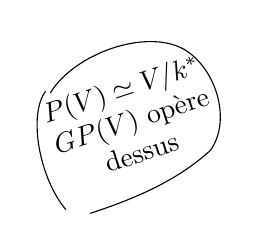
\begin{tikzpicture}[rotate=18,transform shape,baseline=(proj.base)]
\node[inner sep=1pt,align=center] (proj) at (0,0)
  {$\mathbb{P}(V)\simeq V/k^*$\\$\operatorname{GP}(V)$ opère\\dessus};
\draw (-.87,.64) .. controls (-.43,1.02) and (.53,1.05) .. (.91,.65)
  .. controls (1.23,.30) and (1.22,-.40) .. (.84,-.68)
  .. controls (.34,-.91) and (-.24,-.97) .. (-.86,-.97);
\draw (-.92,.68) .. controls (-1.22,.47) and (-1.34,-.33) .. (-1.14,-.83);
\end{tikzpicture}}
\normalmarginpar

Structure de $k$-vectoriel
\tikz[baseline=(vecbase.base)]{
  \node[anchor=base west,inner sep=0pt] (vecbase) at (0,0) {sur ens $V$};
  \node[anchor=base west,inner sep=0pt,font=\scriptsize] at (-.05,.58) {\inserted{de dim $n$}};
  \draw (-.02,-.12) .. controls (-.30,.38) and (-.13,.43) .. (.49,.48)
    .. controls (.99,.54) and (1.63,.48) .. (1.82,.64)
    -- (1.76,.70);
}
$\longleftrightarrow$ donnée d'\unsure{un|une} \unsure{élémt|élément} de $\operatorname{Isom}_{\text{ens}}(k^n,V)/\operatorname{Gl}(n,k)$

Structure de $k$-espace affine de dim $n$ sur \deleted{$E$} ens $E$
\[
\longleftrightarrow\ \text{donnée d'un élément de}\quad
\operatorname{Isom}_{\text{ens}}(k^n,V)/\operatorname{Aff}(n,k)
\]

[ De façon \unsure{général|générale}, \deleted{si $Z$ est un groupe}, la notion de
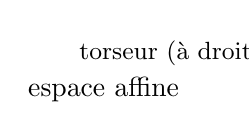
\begin{tikzpicture}[baseline=(oldtor.base)]
  \node[anchor=base west,inner sep=0pt] (oldtor) at (0,0) {\deleted{espace affine}};
  \node[overlay,anchor=base west,inner sep=0pt,font=\small] at (.65,.48)
    {\inserted{torseur (à droite, disons) $E$}};
  \path[use as bounding box] (0,-.08) rectangle (2.45,.88);
\end{tikzpicture}
sous \unsure{grpe|groupe} non précisé peut être considéré comme structure sur le seul ens de base $E$,
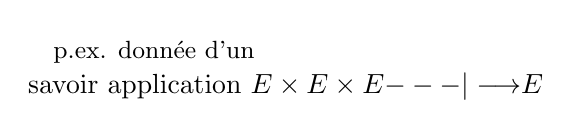
\begin{tikzpicture}[baseline=(oldapp.base)]
  \node[anchor=base west,inner sep=0pt] (oldapp) at (0,0)
    {\deleted{\unsure{savoir application} $E\times E\times E\unsure{\mathbin{\text{---}}|\longrightarrow}E$}};
  \node[overlay,anchor=base west,inner sep=0pt,font=\small] at (.32,.44)
    {\inserted{p.ex. donnée d'un}};
  \path[use as bounding box] (0,-.08) rectangle (6.7,.83);
\end{tikzpicture}
\deleted{$(x,y,z)\longmapsto\unsure{6x|sx}$} couple $\Gamma\subset\mathfrak{S}_{E}$ ss-grpe, tel que \ldots ] ; valable pour ens. à grpe d'op \uline{fidèle}\ldots ]

Une structure d'\uline{espace affine sous} $k$ est alors la donnée d'un tel $\Gamma$, avec \deleted{\unsure{$\Gamma$ com}} comm, \unsure{et|\deleted{et}} un hom d'anneaux unit.
\[
 k\longrightarrow\operatorname{End}_{\mathbb{Z}}(\Gamma)\quad\ldots\qquad ]
\]

Structure de $k$-espace projectif de dim $n$ sur $\unsure{P|\mathbb P}$
\[
\mathrel{\tikz[baseline=(defeq.base)]{
  \node[inner sep=0pt] (defeq) at (0,0) {$\longleftrightarrow$};
  \node[inner sep=0pt,font=\scriptsize] at (0,.71) {déf};
  \draw (-.36,.89) -- (-.36,.48) -- (.27,.48)
    .. controls (.38,.49) and (.40,.65) .. (.40,.88);
  \draw[->] (0,.48) -- (0,.12);
}}
\ \text{donnée de}\quad
\operatorname{Isom}_{\text{\unsure{ens|ens,}}}\left(
 \underset{\substack{\rotatebox{90}{$=$}\\(k^n-(0)/k^*}}{\mathbb{P}^{n-1}(k)},P\right)
 /\operatorname{GP}(n-1,k)
\]

\figure{
\begin{tikzpicture}[x=\linewidth,y=1ex]
\draw (.29,1.5) -- (.58,1.5) .. controls (.61,1.5) and (.61,-.5) .. (.65,-.5) -- (.98,-.5);
\end{tikzpicture}}
\diagram{\begin{tikzcd}[ampersand replacement=\&,column sep=small,row sep=.6em]
\operatorname{Gl}(n,k)\arrow[r]\&\operatorname{Aff}(n,k)\arrow[r]\&\operatorname{GP}(n,k)\\
\substack{\text{vect. de dim $n$}\\\text{sur $k$}}\arrow[r,maps to,"\substack{\text{oubli}\\\text{origine}}"']
\&\substack{\text{espace affine de}\\\text{dim $n$ sur $k$}}
\arrow[r,maps to,"\substack{\text{espace proj.}\\\text{associé à}\\\text{l'esp. vect. \unsure{enveloppant|enveloppe}}}"']
\&\substack{\text{espace projectif}\\\text{de dim $n$ sur $k$}}
\end{tikzcd}}
% archive sheet number: 13
